\section{Benchmark NIST-6 "Boundary Layer"}
\label{sec:bench-6}

This problem has an boundary layer along the right and top sides of the domain.
It is a convection-diffusion equation with first order terms.

\begin{equation} \label{boundary-layer}
-\epsilon \nabla^{2} u + 2\frac{\partial u}{\partial x} + \frac{\partial u}{\partial y}= f
\end{equation}
in the domain $\Omega = (-1, 1)^2$, equipped with Dirichlet boundary condition
given by the exact solution.

The exact solution
\begin{equation}\label{exact-nist-6}
u(x,y) = (1 - e^{-(1 - x) / \epsilon})(1 - e^{-(1 - y) / \epsilon})cos(\pi (x + y))
\end{equation}
where $\epsilon$ determines the strength of the boundary layer.
The right-hand side $f$ is calculated by inserting (\ref{exact-nist-6}) into (\ref{boundary-layer}).
The solution of NIST-6 with $\epsilon = 10^{-1}$ is shown in Fig. \ref{fig:sln-nist06}.

\begin{figure}[!ht]
\centering
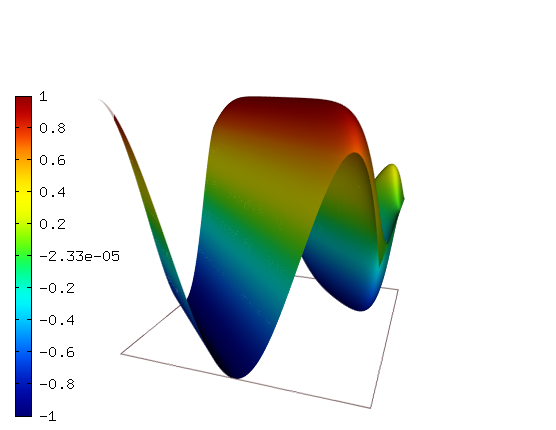
\includegraphics[height=5cm]{nist/nist-6/solution.png}
\caption{The solution to NIST-6 benchmark problem.}
\label{fig:sln-nist06}
\end{figure}
